\apendice{Documentación de usuario}
En esta sección del anexo se han definido aquellos requisitos necesarios para la ejecución y puesta en marcha del proyecto. 
\section{Requisitos software y hardware para ejecutar el proyecto.}
\subsection{Requisitos del software}
Para el correcto funcionamiento es necesario tener instalado en el ordenador todas las herramientas y programas que se han utilizado. 
\begin{itemize}
    \item Python: Este programa es esencial para que el código se ejecute y se abra el desplegable.
    \item Arduino IDE: Este programa es necesario para tener una comunicación y conexión correcta entre la placa de arduino y el ordenador 
    \item Editor de texto/codigo: No es estrictamente necesario la instalación de un editor de texto/codigo como Visual Estudio Code, pero si puede facilitar el uso tanto al usuario como a posibles profesionales ingenieros para la solución de errores.
    \item Instalación de bibliotecas:
    
    - Pandas: manipulación y analisis de datos estructurados(tablas)
    
    -Pyserial: comunicación con puerto serie
    
    -Kivy: paquete que permite la creación de la interfaz gráfica
    
    -kivymd: paquete que permite la creación de la interfaz gráfica

    -Openpyxl: abrir y modificar archivos excel.
    
    

\begin{table}[]
\centering
\begin{tabular}{|l|l|}
\hline
\rowcolor[HTML]{BFBFBF} 
\textbf{Software} & \textbf{Descripción} \\ \hline
Python & Versión 3.13\\ \hline
Arduino IDE & Versión 2.3.6\\ \hline
Bibliotecas & Versiones más actualizadas\\ \hline
\end{tabular}
\caption{Requisitos Software}
\label{tab:Requisitos_Software}
\end{table}
\end{itemize}
\subsection{Requisitos del hardware}
Para el correcto funcionamiento es necesario el uso del dispositivo creado, un ordenador y el cable USB que conecte el ordenador con la placa de Arduino.
\section{Instalación / Puesta en marcha}
\subsection{Python}

El proceso de descargar Python es sencillo. Desde la web oficial de Python \cite{Python}, en la pantalla inicial (ver figura \ref{fig:Python}), aparece un botón de descarga(señalado con una flecha roja). Al seleccionarlo, la descarga se inicia de forma  automática. Una vez descargado el archivo,el proceso de instalación se realiza de una forma similar a la de otras aplicaciones: se decide la ruta de instalación deseada y el programa queda instalado en nuestro ordenador.

\begin{figure}[h]
        \centering
        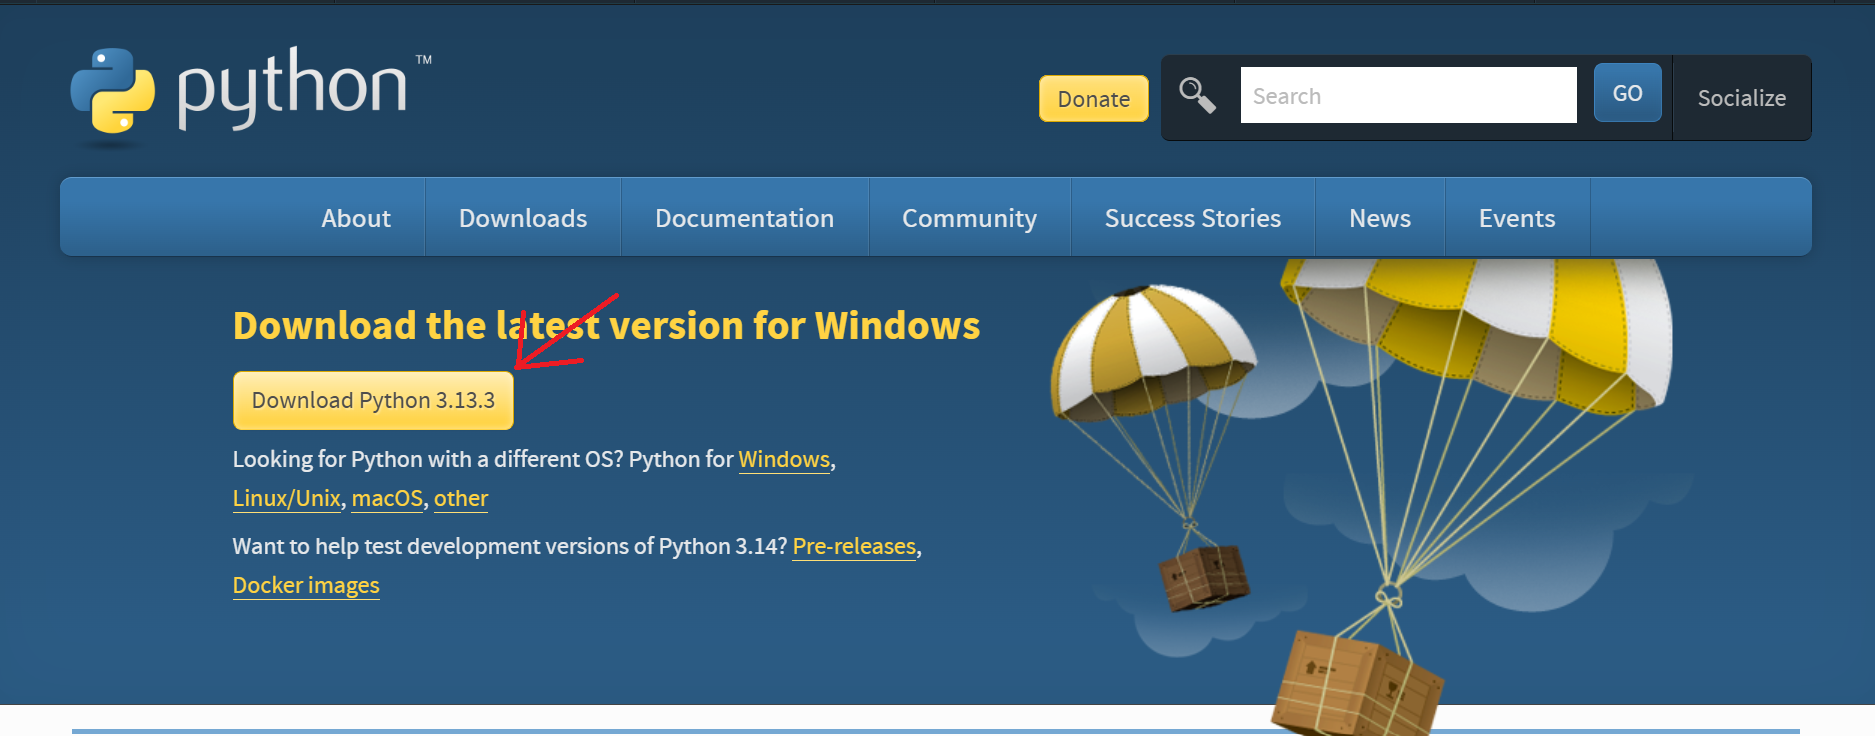
\includegraphics[width=0.8\textwidth]{img/pantalla inicio python.png}
        \caption{pantalla descargar Python}
        \label{fig:Python}
    \end{figure}
\subsection{Arduino IDE}
Proceso muy similar a la instalación de Python.Desde la web oficial de Arduino IDE \cite{Arduino}, en la pantalla inicial (ver figura \ref{fig:Arduino}), aparece una sección de diferentes opciones de descarga según el sistema operativo instalado en el ordenador. Al seleccionar el archivo correspondiente a nuestro sistema operativo, se abre una ventana nueva en la cual hay que clickear el botón 'Just Download' y la descarga se iniciará de forma  automática. Una vez descargado el archivo,el proceso de instalación se realiza de una forma similar a la de otras aplicaciones: se decide la ruta de instalación deseada y el programa queda instalado en nuestro ordenador.
    \begin{figure}[h]
        \centering
        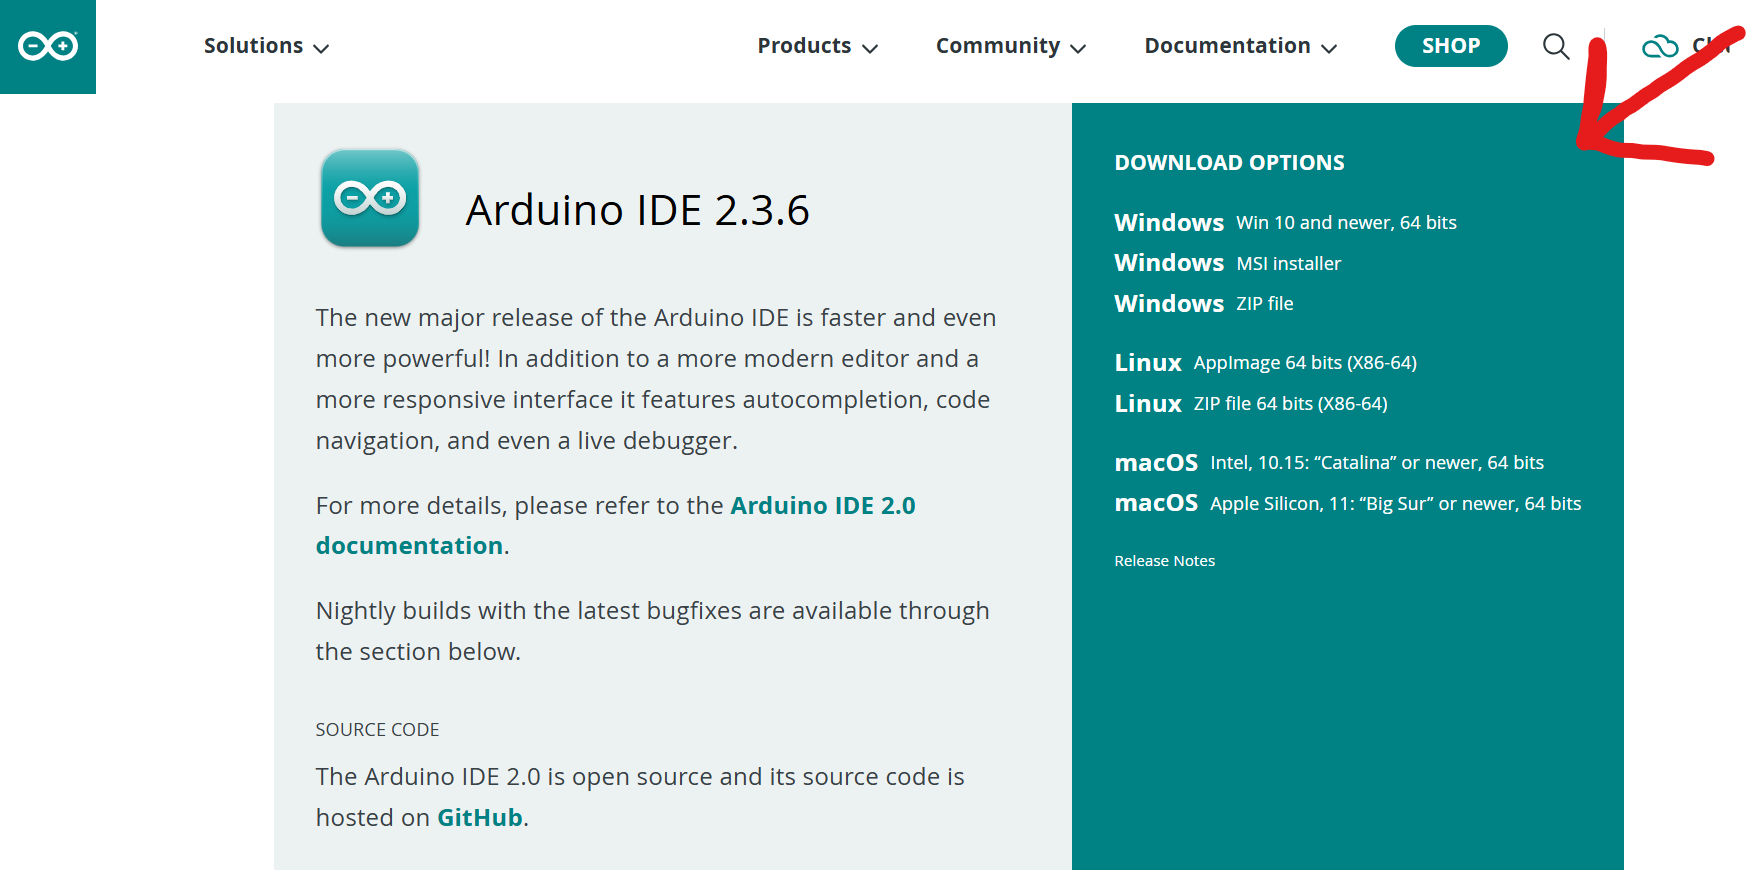
\includegraphics[width=1\textwidth]{img/pantalla inicio arduino IDE.png}
        \caption{pantalla descargar Arduino}
        \label{fig:Arduino}
    \end{figure}
\subsection{Instalación de bibliotecas}
La instalación de las bibliotecas se hace desde la consola del sistema (CMD).Para abrirla, basta con buscar CMD en el buscador de windows y hacer click sobre el resultado.
Una vez abierta la consola (ver figura\ref{fig:CMD}), se deben introducir los siguientes comandos para la instalación de las bibliotecas:

pip install pandas

pip intall pyserial

pip install kivy 

pip install kivymd

pip install openpyxl

\begin{figure}[h]
    \centering
    \includegraphics[width=0.8\textwidth]{img/pantalla CMD.png}
    \caption{pantalla CMD}
    \label{fig:CMD}
\end{figure}
\section{Manuales y/o Demostraciones prácticas}




    
     